\section{Resultat och analys}
Beskriv och förklara slutresultatet. bre Det är viktigt att det visuellt visas upp på bästa sätt i rapporten,
men också att resultaten beskrivs så att läsaren kan förstå hur ni har tänkt och vilka effekter som olika val som ni har gjort har haft på ert slutresultat.
Resultat och förändringar av ert projekt i samband med testning ska också vara med.
\\\\
Resultatet av Projekt Streamline är en användarvänlig och strukturerad webbapplikation byggd i React, vars syfte är att ersätta det tidigare dokumentationssystemet Pelagia har i Excel.
Genom en iterativ process med kontinuerliga tester och dialoger med användarna på Pelagia har applikationen byggts för att bättre möta deras behov. Det levererade systemet blev
ett mer överskådligt, lättanvänt och robust system som förhoppningsvis kan byggas vidare på och effektivisera Pelagias process.
\subsection{Systemets delar}
Det levererade resultatet kan delas upp i tre huvudkomponenter samt en extra vy i form av en statistiksida. Huvudkomponenterna är tillsammans vad som utgör användarupplevlsen
och var det faktiska arbetet sker i applikationen.
\subsubsection{Topbar}
Topbar är placerad högst upp i gränssnittet och visar tabbar för de projekt som användaren för tillfället har öppnat. Den aktiva tabben får vit bakgrund
och extra höjd för att tydliggöra vilket projekt som är aktivt i workspace (se figur \ref{fig:topbar}).
Den fungerar som ett verktyg för att hålla koll på och snabbt kunna växla mellan projekt utan att behöva söka upp dem igen.
Till höger på topbar finns även information om det projekt som för närvarande är aktivt, i syfte att ge en snabb översikt.

\begin{figure}[H]
    \centering
    
\includegraphics[width=1\linewidth]{images/topbar.PNG}
    \caption{Hela topbaren med tre öppna tabbar och ''Projekt A'' som aktivt projekt.}
    \label{fig:topbar}
\end{figure}

\noindent Informationen till höger visar projektets prioritet med färg (grön, gul eller röd),
projektets deadline, antal färdiga prover jämfört med totala antalet, samt antalet kommentarer kopplade till proverna
(se figur \ref{fig:topbar_info}).

\begin{figure}[H]
    \centering
    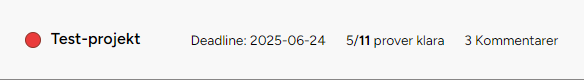
\includegraphics[width=0.8\linewidth]{images/topbar_h_info.PNG}
    \caption{Översiktsinformation om projektet ''Test-projekt'' i topbar.}
    \label{fig:topbar_info}
\end{figure}

\noindent Det går även att byta namn på projektet genom att dubbelklicka på namnet (se figur \ref{fig:topbar_nytt_namn}). 

\begin{figure}[H]
    \centering
    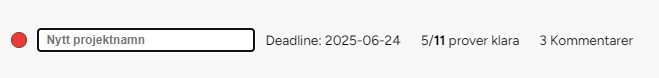
\includegraphics[width=0.8\linewidth]{images/topbar_nytt_namn.PNG}
    \caption{Namnbyte på projekt i topbar genom dubbelklick på nuvarande namn.}
    \label{fig:topbar_nytt_namn}
\end{figure}

\subsubsection{Sidebar}
Sidebar är placerad till vänster på skärmen och fungerar egentligen som en vanlig filhanterare på din dator, den tillåter navigering och organisering av olika filer (projekt i detta fall) och mappar.
Den byggdes på detta sätt för att fylla Pelagias behov att få en tydlig överblick av alla projekt samt att framtidssäkra deras system i form av anpassning,
vilket var svårt med deras tidigare system i Excel.  

\begin{figure}[H]
    \centering
    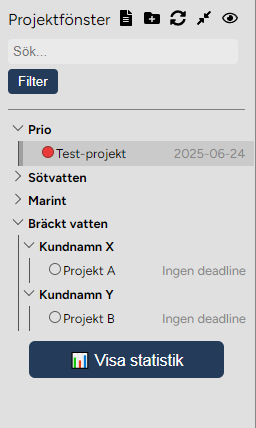
\includegraphics[width=0.5\linewidth]{images/sidebar2.png}
    \caption{Sidebar med projekt och mappar som kan organiseras fritt av användaren.}
    \label{fig:sidebar}
\end{figure}

\noindent Ikonerna uppe till höger i figur \ref{fig:sidebar} är i ordning:
\begin{itemize}
    \item Skapa nytt projekt.
    \item Skapa ny mapp.
    \item Ladda om (tänk uppdatera och hämta om det skett ändringar från annan dator).
    \item Stäng alla öppna mappar.
    \item Göm sidebar.
\end{itemize}

\noindent De första två punkterna på listan ovan är självklara och ett måste, resterande var inte explicit önskade av Pelagia men projektgruppen valde att ha med för att ge flexibilitet.
Funktionen att ladda om är inte implementerad men är tänkt att finnas eftersom systemet kommer köras på flera datorer samtidigt och det ska finnas möjlighet för de som arbetar i labbet att kunna hämta nya projekt som skapats från inskrivningsrummet till exempel.
Det finns argument att istället bygga systemet för att stödja realtidsuppdateringar, dock hade det krävt mycket mer kod och generellt är det inte flera som arbetar på samma ställe i systemet på Pelagia.
Att kunna stänga alla öppna mappar vilket är användbart för att antalet mappar(kunder) i Pelagias fall redan är högt och kommer säkerligen att växa. Knappen för att gömma sidebar har en liknande anledning som att stänga alla mappar, alltså minska antalet saker på skärmen för att arbeta någon annanstans.
\\\\
Det finns även funktionalitet för att döpa om, radera och flytta både projekt och mappar, detta för att ge Pelagia full kontroll av deras struktur och arbetssätt. Flytt av mapp eller projekt görs genom ''drag and drop''. Implementationen av detta är
lite skakig, men syftet är att det ska vara enkelt och intuitivt att flytta något. Namnbyte och radering hittas genom att högerklicka på ett projekt eller mapp och för att förhindra att detta råkas göra, behöver dessa funktioner bekräftas i en ''pop up'' modal innan ändringen tar effekt.
Utöver namnbyte och radering går det att sätta prioritet och deadline på projekt genom högerklick (se figur \ref{fig:sidebar_menu}) vilket var något Pelagia vill ha i sitt system.
\begin{figure}[H]
    \centering
    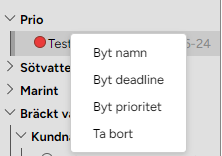
\includegraphics[width=0.5\linewidth]{images/sidebar_menu.png}
    \caption{Högerklicksmeny för projekt i sidebar.}
    \label{fig:sidebar_menu}
\end{figure}
\noindent En ytterligare funktion som lades till var möjligheten till att söka efter projekt och mappar i sidebar, det går direkt att söka efter namn (se figur \ref{fig:sidebar_sok}) eller att använda filterfunktionen om man inte vet exakt namnet på vad man letar efter (se figur \ref{fig:sidebar_filter}).
\begin{figure}[H]  
\centering
    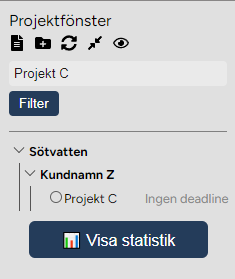
\includegraphics[width=0.5\linewidth]{images/sidebar_sok.PNG}
    \caption{Sökning efter ''Projekt C'' i sidebar och resultat.}
    \label{fig:sidebar_sok}
\end{figure}
\begin{figure}[H]  
\centering
    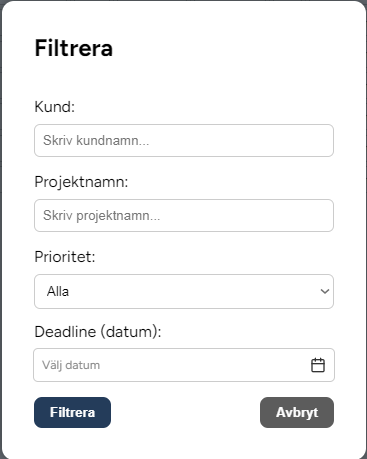
\includegraphics[width=0.5\linewidth]{images/sidebar_filter.PNG}
    \caption{Filterfunktion för sökning i sidebar.}
    \label{fig:sidebar_filter}
\end{figure}

\noindent Slutligen för sidebar, genom att dubbelklicka på ett projekt öppnas motsvarande tabell i workspace och visas i Topbar som en tabb.
Målet med denna struktur har varit att ersätta de stora, ostrukturerade kalkylarken i Excel med ett mer överskådligt och användarvänligt system.
\subsubsection{Workspace}
\subsubsection{Statistiksida}

\subsection{}